\section{Experimental setup}
\label{sec:setup}
The MB events in p--Pb collisions at $\snn$~=~5.02~TeV used for the present analysis are recorded using the ALICE detector in 2016. The center-of-mass reference system in p--Pb collisions is shifted by $\Delta \mathrm{y}_{\mathrm{cms}} =$~0.465 units of rapidity along the direction of the proton beam. In the following, the convention that $\mathrm{y}$ stands for $\mathrm{y}_{\mathrm{cms}}$ is used. The ALICE apparatus used during the LHC Run 2 is described in detail~\cite{Abelev:2014ffa}. The present analysis is carried out using the following detectors: V0~\cite{ALICE:2013axi}, the Zero Degree Calorimeters (ZDC)~\cite{Cortese:2019nnv}, the Inner Tracking System (ITS)~\cite{ALICE:2010tia}, the Time Projection Chamber (TPC)~\cite{Alme:2010ke}, and the Time-Of-Flight (TOF)~\cite{Jacazio:2018slq}. 

The V0 detector is an hodoscope of scintillators, located on both sides relative to the interaction point (IP), consisting of V0A and V0C, each made of 32 plastic scintillator strips, covering the full azimuthal angle within the pseudorapidity intervals $2.8 < \eta < 5.1$ and $-3.7 < \eta < -1.7$, respectively. The MB events are selected with a signal given by a hit in both the V0A and V0C in p--Pb collisions. The V0A on the Pb-going side provides the multiplicity class using the sum of the V0A signals at the same time. The collected MB sample corresponds to an integrated luminosity of 0.24~nb$^{-1}$~\cite{ALICE:2014gvw}. The ZDC in p--Pb collisions detects nucleons emitted from the colliding nucleus by nuclear de-excitation processes or knocked out from wounded nucleons, the so called “slow” nucleons. Two identical sets of the ZDC, each composed by a neutron (ZN) and a proton (ZP) calorimeters, are located at 112.5 m from the ALICE IP, on both sides, covering very forward rapidity regions. The ZDC provides the least biased centrality selection in p--Pb collisions~\cite{ALICE:2014xsp}.

%The V0A detector is utilized to measure the particle yield ratio of \fzero~because the multiplicity dependence of $\mathrm{K}^{*0}$ and $\pi$ yields are measured with the V0A detector. The ZDC which detects ``slow'' nucleons at very large $\eta$~\cite{Cortese:2019nnv}  also defines the most unbiased multiplicity class for the event selection. The multiplicity dependence of the nuclear modification factor of \fzero~is measured using the hybrid method, which can be conducted with the ZDC~\cite{ALICE:2014xsp}, to scale down the cross section of the \fzero~in p--Pb collisions with a reduced bias.

The primary vertex position is reconstructed using the measured track segments in the Silicon Pixel Detector (SPD)~\cite{Santoro2009:ALICESPD}, the innermost two layers of the ITS. The primary vertex along the beam direction ($z_\mathrm{vtx}$) is required to be in $|z_\mathrm{vtx}|<10$~cm from the nominal point ($z_\mathrm{vtx}=0$). One of standard pileup rejections is performed when the longitudinal displacement of multiple primary vertices is larger than 0.8~cm. The probability of pileup events is expected to be 0.5\% in MB events. The TPC is the main tracking detector of ALICE. The TPC covers the pseudorapidity range $|\eta|<$~0.9 over the full azimuth in a uniform solenoidal magnetic field of 0.5~T along the beam axis. The TPC is able to reconstruct charged particles down to $p_{\rm{T}}=$~0.15~GeV/$c$. Particle identification (PID) can be performed with the TPC and TOF. The TPC measures ionization energy loss $\mathrm{d}E/\mathrm{d}x$ of charged tracks to separate particle species. The TOF helps particle identification by measuring the flight time of charged particles from the primary vertex to the TOF.

\section{Data analysis}

The \fzero~is reconstructed via the decay channel of \fzero~$\rightarrow \pi^{+}\pi^{-}$, where the branching ratio is reported as B.R. = $46\pm6$\%~\cite{Stone:2013eaa}. Each charged pion reconstructed in the TPC is required to have $p_{\rm{T}}>$~0.15~GeV/$c$ and $|\eta|<$~0.8 for a uniform detector acceptance. The reconstructed tracks are required to satisfy the standard selection criteria, as reported in~\cite{ALICE:2022qnb}, to guarantee that only tacks with high quality are selected. To ensure good track momentum resolution, the reconstructed tracks are required to have at least 70 reconstructed points (out of a maximum of 159) in the TPC and two hits in the ITS, with at least one in the SPD. Selection criteria dependent on $p_{\mathrm{T}}$ are applied to the distance of closest approach to the primary vertex in the transverse ($d_{z}$) and longitudinal ($d_{xy}$) directions, requiring $d_{z}<$~2~cm and $d_{xy}<$~(0.0105~$+$~0.0350~$\times p_{\mathrm{T}}^{-1.1})$~cm, respectively, to suppress contamination from secondary charged particles originating from weakly decaying hadrons.

The identification of charged pions is performed using the combined information of the TPC and TOF. The difference between the measured ionization energy loss and the prediction of the Bethe-Bloch parameterization obtained assuming the particle is a pion is required to be within two standard deviations to identify pions using the TPC. The difference between the measured time-of-flight of the particle and the time expected for a pion is required to be within three standard deviations to identify pions using the TOF. The TOF is not used for the particle identification when the TOF signal is expected not to be originating from the reconstructed track, and the TPC is used for the identification as a standalone detector.

\label{sec:ana}
\begin{figure}[hbt!]
	\centering
	\subfigure{ 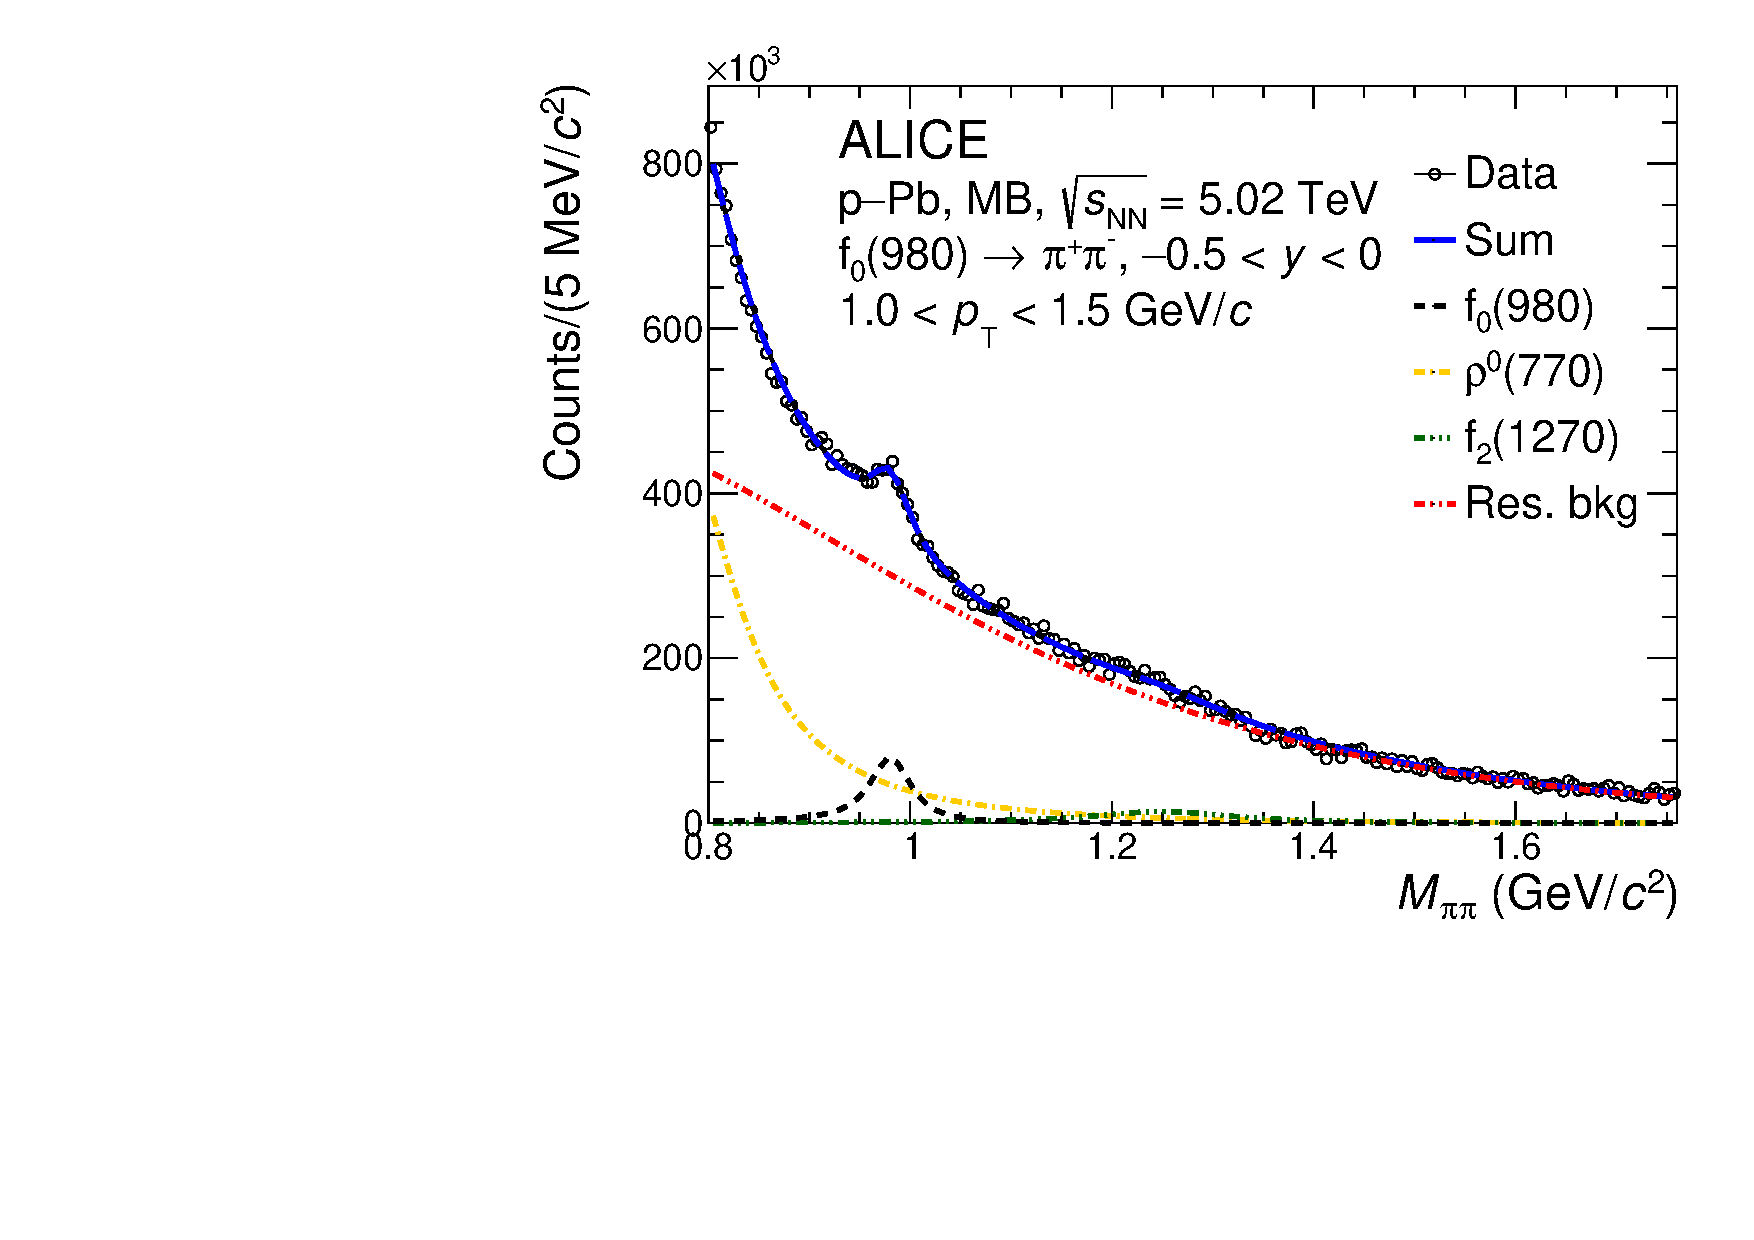
\includegraphics[width=0.47 \textwidth]{figures/Fig1_sigext_mb_pt0.pdf} }
	\subfigure{ 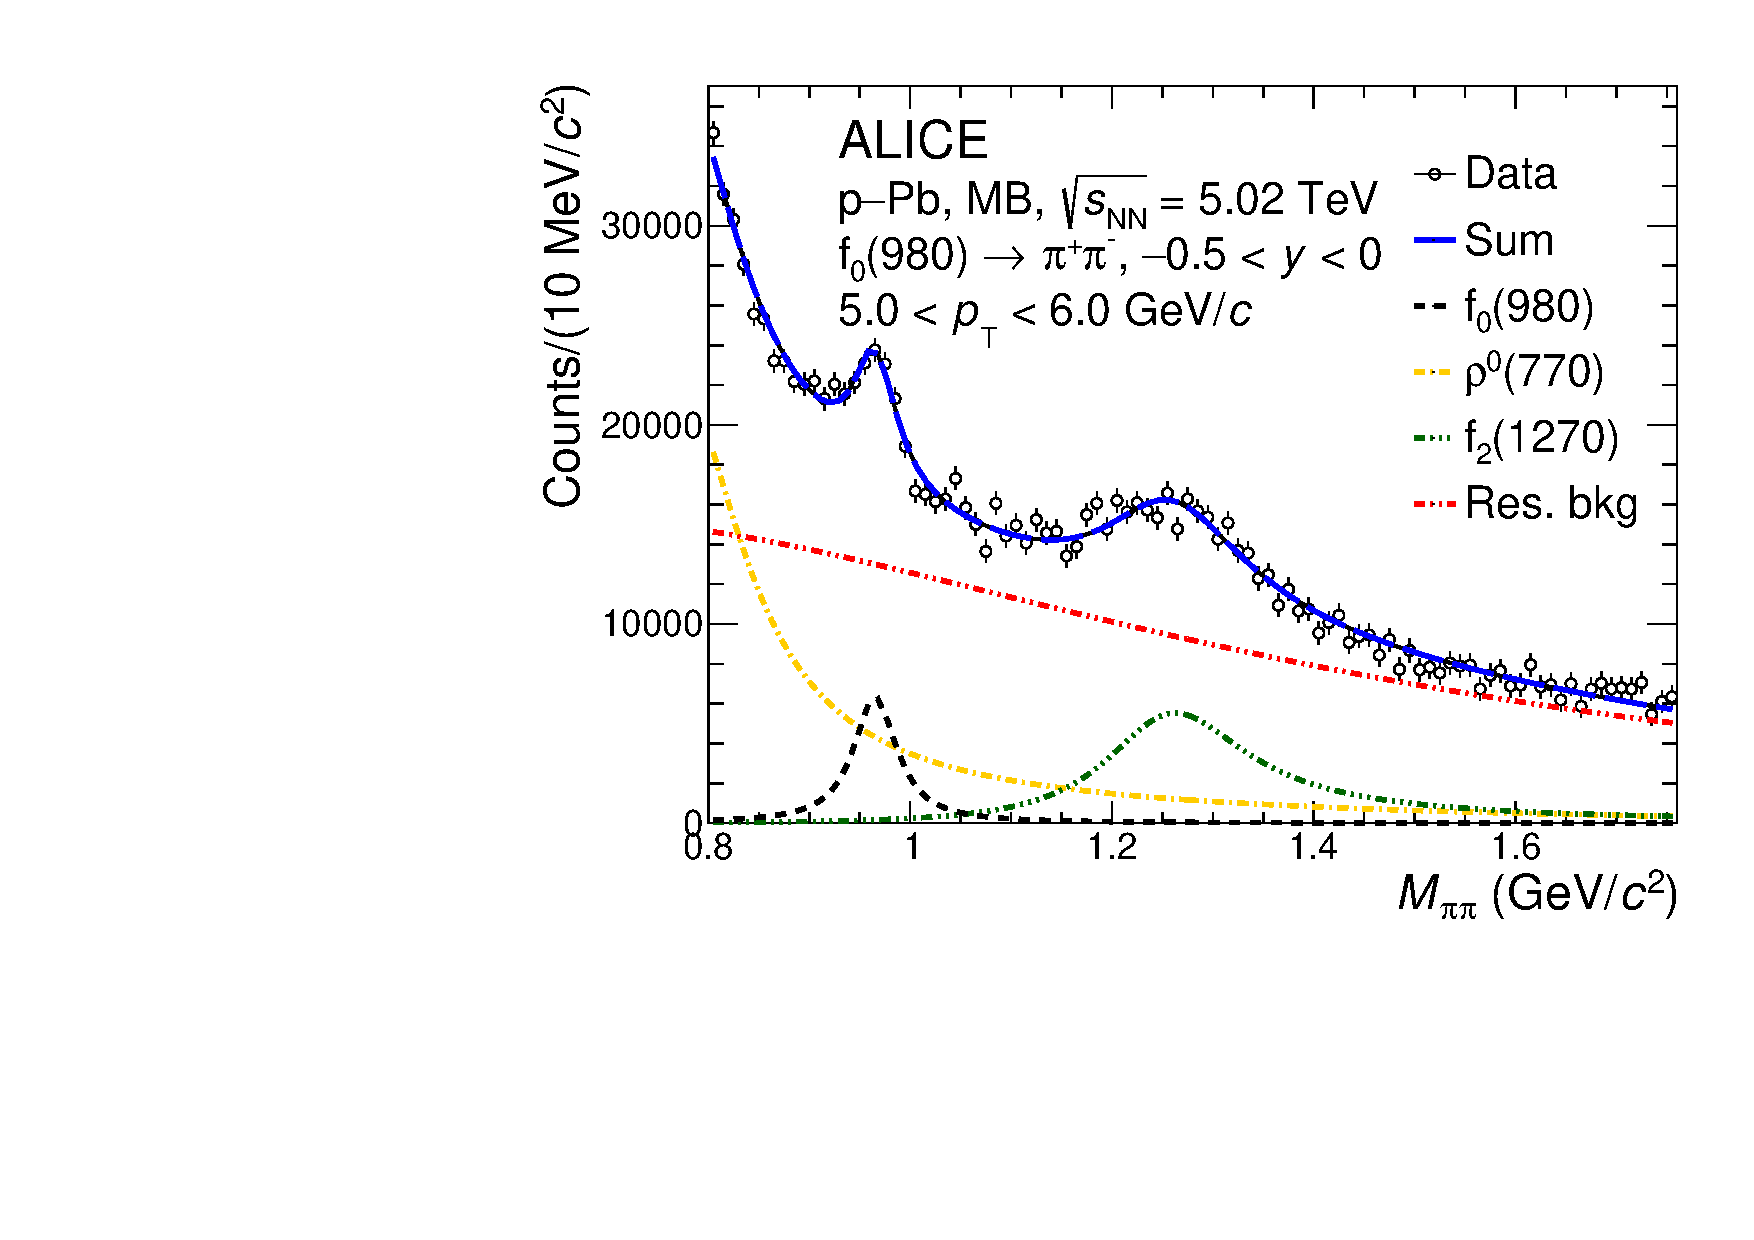
\includegraphics[width=0.47 \textwidth]{figures/Fig1_sigext_mb_pt1.pdf} }
	\caption{ Invariant mass distribution of $\pi^{+}\pi^{-}$ pairs in $-0.5<\mathrm{y}<0$ after the like-sign background subtraction in p--Pb collisions at \snn~=~5.02~TeV. The left (right) plot is obtained at low (high) $p_{\mathrm{T}}$ of $\pi^{+}\pi^{-}$ pairs in non-single diffraction (NSD) events. }
	\label{fig:SigExt}
\end{figure}

The \fzero~signals are extracted using the invariant mass analysis by associating oppositely-charged two pions in the same event at -0.5~$<\mathrm{y}<$~0~\cite{ALICE:2013wgn}. The combinatorial backgrounds are subtracted using the like-sign method~\cite{PhysRevD.36.2019}. The like-sign backgrounds are constructed as the geometric average of $\pi^{+}\pi^{+}$ and $\pi^{-}\pi^{-}$ distributions,  2$\sqrt{N_{\pi^{+}\pi^{+}}N_{\pi^{-}\pi^{-}}}$. After subtracting the like-sign backgrounds from $\pi^{+}\pi^{-}$ distribution, peaks of resonances decaying to $\pi^{+}\pi^{-}$ can be identified. Figure~\ref{fig:SigExt} shows the like-sign-subtracted $\pi^{+}\pi^{-}$ invariant mass distributions for 1.0~$<p_{\rm{T}}<$~1.5~GeV/$c$ (5.0~$<p_{\rm{T}}<$~6.0~GeV/$c$) in MB events on the left (right) plot. Because $\rho$(770) and $\rm{f}_{2}$(1270) dominantly decay to $\pi^{+}\pi^{-}$ and have large widths, \fzero~signals are overlapped with contributions from those two resonances. Residual backgrounds ($f_{\mathrm{bkg}}$) are mainly attributed to misidentified particles and mini-jets, which are represented as red-dashed-dotted lines in Fig.~\ref{fig:SigExt}. Each resonance contribution is described with a relativistic Breit-Wigner function (rBW)~\cite{ALICE:2018qdv, ALICE:2022qnb}. Note that detector resolution is expected to be negligible for the rBW to estimate the large particle widths of resonances. The rBW can be expressed as
\begin{eqnarray}
\mathrm{rBW}(M_{\pi\pi}) = \dfrac{AM_{\pi\pi}\Gamma(M_{\pi\pi})M_{0}}{(M_{\pi\pi}^{2}-M_{0}^{2})^{2} + M_{0}^{2}\Gamma^{2}(M_{\pi\pi})},
\label{eq:rBW}
\end{eqnarray}
where $\Gamma(M_{\pi\pi})$ is defined as
\begin{eqnarray}
\Gamma(M_{\pi\pi}) = \left[ \dfrac{ (M_{\pi\pi}^{2} - 4m_{\pi}^{2}) }{ (M_{0}^{2}-4m_{\pi}^{2}) } \right]^{(2J+1)/2} \times \dfrac{\Gamma_{0}M_{0}}{M_{\pi\pi}} .
\label{eq:rBWW}
\end{eqnarray}
Here, $A$ and $M_{0}$ are the amplitude of the rBW and the rest mass of the resonance, respectively. The rest width of the resonance, the spin, and the charged pion mass of 139.5~MeV/$c^{2}$ is represented as $\Gamma_{0}$, $J$, and $m_{\pi}$, respectively. The spins for \fzero, $\rho$(770), and $\mathrm{f}_{2}$(1270) are 0, 1, and 2, respectively. The $f_{\mathrm{bkg}}$ is fitted with a Maxwell-Boltzmann-like distribution, which can be expressed as~\cite{OPAL:1998enc}
\begin{eqnarray}
f_{\mathrm{bkg}}(M_{\pi\pi}) = B(M_{\pi\pi}-2m_{\pi})^{n}\exp{(c_{1}M_{\pi\pi} + c_{2}M_{\pi\pi}^{2})},
\label{eq:bkg}
\end{eqnarray} 
where, $B$, $n$, $c_{1}$, and $c_{2}$ are free parameters. Each rBW of the resonance is corrected for the $\pi\pi$ interference~\cite{Rapp:2003ar}, which can be expressed as
\begin{eqnarray}
\mathrm{PS}(M_{\pi\pi}) = \dfrac{M_{\pi\pi}}{\sqrt{M_{\pi\pi}^{2}+p_{\mathrm{T}}^{2}}}\times\exp{(-\sqrt{M_{\pi\pi}^{2}+p_{\mathrm{T}}^{2}}/T_{\mathrm{kin}})},
\label{eq:ps}
\end{eqnarray} 
where $p_{\mathrm{T}}$ in the above equation denotes the transverse momentum of the $\pi\pi$ pair. $T_{\mathrm{kin}}$ is the kinetic freeze-out temperature and set to be 160~MeV~\cite{ALICE:2018qdv} for different multiplicity classes.

The signal extraction carefully considers the width of the \fzero~as the width is not well known yet (10~$<\Gamma_{0}^{\mathrm{f}_{0}}<$~100~MeV/$c^{2}$~\cite{ParticleDataGroup:2020ssz}). The total fit function consists of the sum of three rBWs and $f_{\mathrm{bkg}}$, which is constructed with nine fit parameters. The nine fit parameters consist of 4 parameters for $f_{\mathrm{bkg}}$, mass and width of \fzero, and amplitudes of three resonances. The masses and widths of $\rho$(770) and $\mathrm{f}_{2}$(1270) are well defined in Ref.~\cite{ParticleDataGroup:2020ssz}, and those are fixed to $m_{\rho}=$~775.3~MeV/$c^{2}$, $\Gamma_{\rho}=$~~149.1~MeV/$c^{2}$, $m_{\mathrm{f}_{2}}=$~1,275.5~MeV/$c^{2}$, and $\Gamma_{\mathrm{f}_{2}}=$~186.7~MeV/$c^{2}$ during all fit procedures. Due to the many free parameters during the fit, the procedure is split into three steps to prevent fit results from being in local minima. The purpose of the first step is to obtain unbiased \fzero~width, initial \fzero~width. The first step is only performing using MB events for the whole $p_{\mathrm{T}}$ measured interval to be less affected by statistical fluctuations. During the first step, all parameters are left free. The second step aims at constraining the $f_{\mathrm{bkg}}$. In the second step, the \fzero~width is fixed with the value, determined in the first step. The last fit procedure is processed with the fixed $f_{\mathrm{bkg}}$, while the \fzero~width is set free in the range of 10~$<\Gamma_{0}^{\mathrm{f}_{0}}<$~100~MeV/$c^{2}$. In each step, the fit range is set to 0.8~$<M_{\pi\pi}<$~1.76~GeV/$c^{2}$.

While for the \fzero~analysis performed in pp collisions~\cite{ALICE:2022qnb} the width is constrained to be 55 MeV/$c^{2}$, the present analysis sets the \fzero~width free. In the previous analysis, there is no phase space correction expressed in Eq~\ref{eq:ps}. On the other hand, the present analysis considers the phase space correction for possibly larger $\pi\pi$ interference~\cite{STAR:2003vqj}. It is found that consistent invariant yields are obtained from different analysis methods.

The raw \fzero~yields ($N_{\mathrm{f}_{0}}$) are obtained by integrating the \fzero~rBW in the measured $p_{\mathrm{T}}$ range and corrected for the acceptance, the tracking efficiency, and the PID efficiency and normalized for the event selections and the B.R.~\cite{Stone:2013eaa}, and the fully corrected yield can be expressed as
\begin{eqnarray}
\dfrac{1}{N_{\mathrm{NSD}}}\dfrac{\mathrm{d}^{2}N}{\mathrm{dyd}p_{\mathrm{T}}} = \dfrac{1}{N_{\mathrm{evt}}} \dfrac{ N_{\mathrm{f}_{0}} }{ \Delta \mathrm{y} \Delta p_{\mathrm{T}} } \dfrac{  \epsilon_{\mathrm{trig}} f_{\mathrm{vtx}} f_{\mathrm{S.L.}} }{\mathrm{Acc} \times \epsilon \times \mathrm{B.R.} }.
\end{eqnarray}
Here, $N_{\mathrm{evt}}$ is the number of events satisfying event selection criteria in the specific multiplicity class. The rapidity interval of 0.5 is represented as $\Delta \mathrm{y}$. Coefficients for the acceptance ($\mathrm{Acc}$) and the tracking and the PID efficiency ($\epsilon$) are estimated from a detailed simulation for the ALICE detector responses. The p--Pb events are simulated using the DPMJET~\cite{Fedynitch:2015kcn} event generator with the artificial injection of \fzero~signals. Signals and backgrounds are transported through the detector using GEANT3~\cite{Brun:1994aa}. The $\mathrm{Acc}\times\epsilon$ is estimated to be 26\% at 0~$<p_{\mathrm{T}}<$~0.3~GeV/$c$ and gradually increasing up to 60\% as $p_{\mathrm{T}}$ increases and it is not dependent on the multiplicity class. $\mathrm{B.R.}$ is the branching ratio of the \fzero~$\rightarrow \pi^{+}\pi^{-}$ decay channel. The \fzero~yield is normalized for the trigger efficiency ($\epsilon_{\mathrm{trig}}$), vertex reconstruction efficiency ($f_{\mathrm{vtx}}$), and signal loss ($f_{\mathrm{S.L.}}$) due to the event selection. The $\epsilon_{\mathrm{trig}}$ is estimated to be dependent on the multiplicity class and to increase from 0.84 to 1 as the multiplicity increases. The $f_{\mathrm{vtx}}$ is estimated to be larger than 0.99 in all measured multiplicity classes. Because current realistic simulations rarely produce primary \fzero, the $f_{\mathrm{S.L.}}$ is estimated using a different particle, the $\phi$ meson, exploiting the universal $m_{\mathrm{T}}$ scaling~\cite{Altenkamper:2017qot}. This approach shows the $f_{\mathrm{S.L.}}$ does not depend on particle species~\cite{ALICE:2019xyr}. The $f_{\mathrm{S.L.}}$ is 1.03 for 0~$<p_{\mathrm{T}}<$~0.3~GeV/$c$ and saturates at unity for $p_{\mathrm{T}}>$~2~GeV/$c$.

\section{Systematic uncertainties}
\label{sec:syst}
The systematic uncertainties of invariant yields are estimated by varying the analysis selection criteria and corrections and are summarised in Tab.~\ref{tab:syst}. The total systematic uncertainty is calculated as the sum in quadrature of the different contributing sources. Each uncertainty does not significantly depend on the chosen $p_{\rm{T}}$ range and the multiplicity class.

\begin{table}[h!]
\caption{The relative systematic uncertainty of invariant $p_{\rm{T}}$-differential yields. Numbers given in ranges correspond to minimum and maximum uncertainties.}
\centering
\begin{tabular}{ll|c}
\hline 
\multicolumn{2}{c|}{Sources}  &Systematic uncertainty (\%) \\ \hline
\multicolumn{2}{l|}{Primary vertex} & negligible \\ 
\multicolumn{2}{l|}{Tracking} & $\pm$4--6 \\
\multicolumn{2}{l|}{Particle identification} & $\pm$4--12 \\ 
\multirow{4}{*}{Signal extraction} &  $\mathrm{f}_{2}$(1270) parameters	& $\pm$3--9 \\ 
& $\rho$(770) parameters & $\pm$3--8 \\
& Fit range & $\pm$0--6 \\
& Initial $\mathrm{f}_{0}$ width & $\pm$2--12 \\
\multicolumn{2}{l|}{Phase space correction} & $\pm$3--8 \\ \hline 
\multicolumn{2}{c|}{Total (in quadrature)}	& $\pm$15--27 \\ 
\hline 
\end{tabular}
\label{tab:syst}
\end{table}

The systematic uncertainty from the primary vertex selection is tested by narrowing the requirement to 7~cm, and the uncertainty is estimated to be negligible. The systematic uncertainty from the pileup rejection is tested by varying the minimal number of track segments contributing to the reconstruction of pileup event vertices from 5 to 3, and the uncertainty is estimated to be negligible.

The systematic uncertainty from tracking is assigned as the value from~\cite{ALICE:2013wgn}, where uncertainties are evaluated by varying the requirements to select reconstructed tracks such as $d_{xy}$, $d_{z}$, and the number of fired TPC readout channels. The systematic uncertainty from the particle identification is tested with different requirements on the number of standard deviations ($\pm\,0.5\sigma$) for the TPC and the TOF, and the uncertainties are estimated to be 4--12\%.

The systematic uncertainties from masses and widths of $\mathrm{f}_{2}$(1270) and $\rho$(770) are evaluated by shifting the masses and the widths, three times within their uncertainties, which are reported at Ref~\cite{ParticleDataGroup:2020ssz}. The estimated uncertainties from $\mathrm{f}_{2}$(1270) and $\rho$(770) parameters are 3--9\% and 3--8\%, respectively. The systematic uncertainty from the fit range is estimated by changing the range inward or outward as much as 40~MeV/$c^{2}$. The uncertainties are estimated to be 
less than 6\%.

The systematic uncertainty from the initial value for \fzero~width, which is obtained in the first step described in Sec.~\ref{sec:ana}, is estimated by varying the width within the statistical uncertainties in both directions. The changes affect the background distribution determined in the second step, and the estimated systematic uncertainties are 2--12\%. The systematic uncertainty from phase space correction is estimated by varying the kinetic freeze-out temperature in the range of 140~$<T_{\mathrm{kin}}<$~180~MeV. The estimated uncertainties are 3--8\%. 

The multiplicity-dependent correlations of systematic uncertainties are evaluated by quantifying how much uncertainties collectively vary in the same direction. The quantification is done by comparing the direction of systematic deviations in the specific multiplicity class and the MB class. Total uncorrelated systematic uncertainties are about half of the total systematic uncertainties for all inspected sources.




\begin{comment}
The systematic uncertainties of invariant yields and \fzero~widths are estimated by varying the analysis selection criteria and corrections, which are summarized in Tab.~\ref{tab:syst}.

The systematic uncertainty from the primary vertex selection is tested by narrowing the requirement to 7~cm and the uncertainty is estimated to be negligible. The systematic uncertainty from the pileup rejection is tested by varying the minimal number of track contributors required for reconstruction of pileup event vertices from 5 to 3 and the uncertainty is estimated to be negligible.

The systematic uncertainty from tracking is assigned as the value from~\cite{ALICE:2013wgn} and the systematic uncertainty from the particle identification is tested with different requirements on the number of standard deviations by $\pm\,0.5\sigma$ for the TPC and the TOF, and the uncertainties are estimated to be 4--12\% for invariant yield and 5--10\% for width.

The systematic uncertainties from masses and widths of $\mathrm{f}_{2}$(1270) and $\rho$(770) are evaluated by shifting the masses and the widths as much as three times their measured statistical uncertainty. The estimated uncertainties for $\mathrm{f}_{2}$(1270) ($\rho$(770)) parameters are 3--9\% (3--8\%) and 2--7\% (2--8\%) for the mass and the width, respectively. The systematic uncertainty from the fit range is estimated by changing the range inward or outward as much as 40~MeV/$c^{2}$. The uncertainties are estimated to be 0--6\% for the yield and 0--5\% for the width.

On the other hand, the width of \fzero~is roughly defined in~\cite{ParticleDataGroup:2020ssz} so that \fzero~width is set to free parameter and estimated in the fit procedure. The systematic uncertainty from the fit range is tested with different fit ranges and estimated to be 2\% at the low $p_{\rm{T}}$ and 8\% at the high $p_{\rm{T}}$. The phase space correction~\cite{Rapp:2003ar} is applied to each rBW to consider possible $\pi\pi$ scattering effects. The temperature of the phase space correction is set to 160 MeV~\cite{ALICE:2013wgn} and the systematic uncertainty from the phase space correction is evaluated with different temperatures and estimated to be 3--8\%. The background function is determined with the pre-fit procedure, which corresponds to the first step in Sec.~\ref{sec:ana}. In the pre-fit procedure, the \fzero~width is fixed as the initial \fzero~width. The systematic uncertainty from the background function is evaluated by varying the initial \fzero~width as much as their measured statistical uncertainties. The uncertainties are estimated to be 8\% at the low $p_{\rm{T}}$ and 3\% at the high $p_{\rm{T}}$.
\end{comment}